\section{Background}

\subsection{The Process Confinement Problem}

The \textit{process confinement problem}, also known as the \textit{sandboxing problem}, refers to the goal of isolating a process or group of processes from the rest of the running system. In practice, this is often achieved by restricting an application's possible behaviour to its desired functionality, explicitly targeting its access to security-sensitive system resources such as files, network interfaces, and other running applications.  Despite decades of work following Lampson's \cite{lampson1973_a_note} first proposal of the process confinement problem in 1973, process confinement remains a somewhat open problem to date \cite{crowell2013_confinement_problem}.

Anderson's 1972 introduction of the reference monitor architecture \cite{anderson1973_planning_study}  has informed the design and implementation of operating system access control mechanisms for nearly five decades. As subjects request access to system resources, the kernel's reference monitor validates requests and makes policy decisions. While all commodity operating systems support at least a basic notion of access control, many implement a coarse-grained, discretionary access control mechanism that is insufficient for providing the fine-grained protection required in security-sensitive or multi-tenant environments. For additional protection, we must turn to more advanced security features offered by the operating system.

A separate yet related problem involves constructing policy languages with which to express security policy. These policy languages need to offer a careful balance of terseness and expressiveness. A policy language must be terse enough to enable human policy authorship and audit yet expressive enough to enforce least-privilege. Similarly, careful consideration is required when developing policy language abstractions. Close conformity with the system's underlying semantics may improve policy expressiveness but impact usability. Significant abstractions might similarly impact the expressiveness of the policy language.

These issues of policy enforcement and policy language design are at the heart of the process confinement problem. This paper seeks to tackle this problem from the perspective of containers and container management.

\subsection{Low-Level Isolation Techniques}
\label{subsection:low_level}

The Linux kernel supports various lower-level abstractions for implementing virtualization and enforcing least-privilege. While many of these mechanisms are insufficient for a full confinement implementation on their own, they are typically used in \textit{combination} by higher-level techniques such as containers (c.f.~\Cref{subsection:containers}) to achieve confinement. This section covers these low-level abstractions in detail.

\todo{Go over each of the following subsections, since they are mostly unchanged from the literature review}

\paragraph*{Unix Discretionary Access Control}

Discretionary access control (DAC) forms the most basic access control mechanism in many operating systems, including popular commodity operating systems such as Linux, macOS, and Windows.  First formalized in the 1983 Department of Defense standard \cite{orange_book}, a DAC system partitions system objects (e.g.~files) by their respective owners and allows resource owners to grant access to other users, at their discretion.  Typically, systems implementing discretionary access control also provide an exceptional user or role with the power to override discretionary access controls, such as the superuser (i.e.~\texttt{root}) in Unix-like operating systems and the Administrator role in Windows.

While discretionary access controls themselves are insufficient to implement proper process confinement, they form the basis for the bare minimum level of protection available on many operating systems; therefore, they are an important part of the process confinement discussion. In many cases, user-centric discretionary access controls are abused to create per-application \enquote{users} and \enquote{groups}. For instance, a common pattern in Unix-like systems such as Linux, macOS, FreeBSD, and OpenBSD is to have specific users reserved for security-sensitive applications such as network-facing daemons. The Android mobile operating system takes this one step further, instead assigning an application- or developer-specific UID (user ID) and GID (group ID) to \textit{each} application installed on the device \cite{android_security}.

In theory, these abuses of the DAC model would help mitigate the potential damage that a compromised application can do to the resources that belong to other users and applications on the system. However, due to DAC's discretionary nature, nothing prevents a given user from granting permissions to all other users on the system, unless other measures are put in place. Further, the inclusion of non-human users into a user-centric permission model may result in a disparity between an end-user's expectations and the reality of what a \enquote{user} is. This gap in understanding could result in further usability and security concerns.

\paragraph*{POSIX Capabilities}

Related to discretionary access control are POSIX capabilities \cite{posix_capabilities,corbet2006_capabities_a,corbet2006_capabities_b}, which can be used to grant additional privileges to specific processes, overriding existing discretionary permissions. Further, a privileged process may \textit{drop} specific capabilities that it no longer needs, retaining those it needs. Consequently, POSIX capabilities provide a finer-grained alternative to the all-or-nothing superuser privileges required by certain applications. For instance, a web-facing process that requires access to privileged ports has no business overriding file permissions. POSIX capabilities provide an interface for making such distinctions. Despite these benefits, POSIX capabilities have been criticized for adding additional complexity to an increasingly complex Linux permission model \cite{corbet2006_capabities_b,corbet2006_capabities_a}.  Further, POSIX capabilities do nothing to confine processes beyond the original DAC model---rather, they help to solve the problem of overprivileged processes by limiting the privileges that they require in the first place.

\paragraph*{Namespaces and Cgroups}

In Linux, \textit{namespaces} and \textit{cgroups} (short for control groups) allow for further confinement of processes by restricting the system resources that a process or group of processes is allowed to access. Namespaces isolate access by providing a process group a private, virtualized naming of a class of resources, such as process IDs, filesystem mountpoints, and user IDs. As of version 5.6, Linux supports eight distinct namespaces, depicted in \Cref{tab:namespaces}.  Complementary to namespaces, cgroups limit the use of \textit{quantities} of system resources, such as CPU, memory, and block device I/O.  Namespaces and cgroups provide fine granularity for limiting a process's view of available system resources. In this sense, they are better classified as a mechanism for implementing virtualization rather than least-privilege. They thus must be combined with other measures to constitute a full confinement implementation.

\begin{table}
\begin{tabular}{lp{3in}}
    \toprule
    Namespace & Isolates \\
    \midrule
    \multirow{1}{*}{PID} & Process IDs (PIDs)\\
    \multirow{1}{*}{Mount} & Filesystem mountpoints\\
    \multirow{1}{*}{Network} & Networking stack\\
    \multirow{1}{*}{UTS} & Host and domain names\\
    \multirow{1}{*}{IPC} & Inter-process communication mechanisms\\
    \multirow{1}{*}{User} & User IDs (UIDs) and group IDs (GIDs)\\
    \multirow{1}{*}{Time} & System time\\
    \multirow{1}{*}{Cgroup} & Visibility of cgroup membership\\
    \bottomrule
\end{tabular}
\caption{Linux namespaces (as of kernel version 5.6) and what they can be used to isolate.}
\label{tab:namespaces}
\end{table}

\paragraph*{System Call Interposition}

System call interposition has historically been a prevalent process confinement technique. Several frameworks exist today for system call interposition on various Unix-like operating systems \cite{anderson2017_comparison, padala2002_ptrace, watson2010_capsicum, pledge}.  Since system calls are used to request services from the operating system, they define the interface with the operating system's reference monitor  \cite{anderson1973_planning_study}. This property makes system call interposition a particularly attractive technique for the implementation of fine-grained policy enforcement mechanisms.

One of the earliest forays into system call interposition for process confinement was TRON \cite{berman1995_tron}. Implemented in 1995 for the Unix operating system, TRON provided a kernelspace mechanism for enforcing \textit{protection domains} on userspace processes. A TRON protection domain consists of its confined processes, a set of allowed operations, and a \textit{violation handler}, which TRON invokes on policy violations. Processes configure protection domains and then employ a special \texttt{tron\_fork} system call to spawn a confined child process. While TRON is not application transparent by itself, it does come with a set of userspace tools to abstract away the configuration of protection domains. Unfortunately, even with these higher-level userspace tools, TRON still assumes a certain degree of security expertise for a user to confine their applications properly.

Perhaps the most pervasive framework for interposing on system calls is ptrace \cite{padala2002_ptrace}, a process tracing and debugging framework that comes enabled in some form or another on all Unix-like operating systems.  While ptrace itself is \textit{not} designed process confinement, some research prototypes \cite{goldberg96_janus, wagner1999_janus} have leveraged it in the past. Unfortunately, ptrace is not generally considered production-safe due to its high overhead and buggy interactions with more complex programs such as sendmail, which is especially problematic considering that these are the types of programs that we often wish to confine.

Janus \cite{goldberg96_janus,wagner1999_janus} was an early exploration of process confinement using Solaris' version of ptrace. In Solaris, ptrace provides a library call interface into the procfs virtual file system and allows tracer applications to make filtering decisions on behalf of traced processes while interposing on system calls. Janus was later ported to Linux using a modified version of Linux's \texttt{ptrace(2)} system call \cite{wagner1999_janus}. In Janus, a supervisor process reads a policy file and attaches itself to a confined process with ptrace. From there, security-sensitive system calls in the confined application are forwarded to the Janus supervisor process to make a policy decision. However, this approach adds considerable overhead to confined processes because ptrace requires \textit{multiple} context switches between userspace and kernelspace to coordinate between the tracer and tracee.

To implement its policy language, Janus defines higher-level interfaces into various groups of system calls, called \textit{policy modules}. These policy modules can filter groups of related system calls by parameterizing them with allowed actions and system objects. While this abstraction is helpful to group system calls by their related functionality, it does little to help Janus' usability, which is still tightly coupled with the underlying system calls. This lack of usability makes it difficult for a non-expert user to write an effective Janus policy.

Anderson published a study in the FreeBSD journal \cite{anderson2017_comparison} comparing three system call interposition frameworks for three distinct Unix-like operating systems: Linux's seccomp-bpf \cite{seccomp_bpf, drewry2012_seccomp_bpf}, OpenBSD's pledge \cite{pledge}, and FreeBSD's Capsicum \cite{capsicum, watson2010_capsicum}. While these three frameworks all interpose on system calls, they do so with varying degrees of security, complexity, and granularity \cite{anderson2017_comparison}, so each merits study in its own regard.

%\begin{figure}[htpb]
%    \centering
%    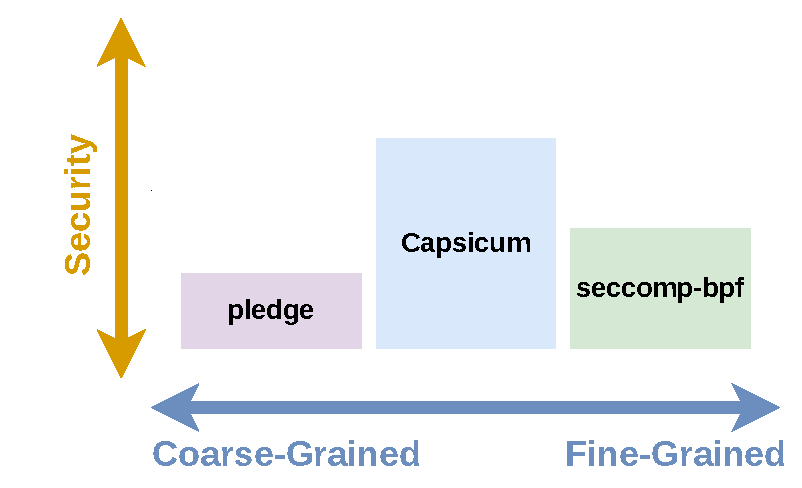
\includegraphics[width=0.8\linewidth]{figs/systemcall-interposition.pdf}
%    \caption{Security and granularity trade-offs of pledge,
%    Capsicum, and seccomp-bpf.}%
%    \label{fig:syscall_interposition}
%\end{figure}

In the original Linux seccomp implementation, processes use a special \texttt{seccomp(2)} system call to enter a secure computing state. By default, processes that have entered this state are restricted to performing \texttt{read(2)}, \texttt{write(2)}, \texttt{sigreturn(2)}, and \texttt{exit(2)} system calls.  Pragmatically, this means that a process could read and write on its open file descriptors, return from invoked signal handlers, and terminate itself. All violations of this policy would result in forced termination. In a 2012 RFC \cite{drewry2012_seccomp_bpf}, Drewry introduced an extension to seccomp enabling the use of BPF programs for the defining filters on system call arguments. This extension, dubbed seccomp-bpf, enables creating fine-grained seccomp policies that filter on system call numbers and arguments, providing a high degree of control to applications that wish to sandbox themselves.

Despite the high degree of control that seccomp-bpf offers to applications, it has severe usability and security concerns, rendering it an unacceptable solution for ad-hoc confinement by end-users. Classic BPF \cite{mccanne1993_bpf} is a rather arcane bytecode language, and writing Classic BPF programs by hand is a task left only to expert users. Further, seccomp-bpf policy is easy to misconfigure, resulting in potential security violations; for instance, an attacker may entirely circumvent a policy that specifies restrictions on the \texttt{open(2)} system call but not \texttt{openat(2)}. Finally, despite userspace library efforts to abstract away the underlying BPF programs \cite{libseccomp}, seccomp-bpf remains accessible only to application developers with significant security expertise.

OpenBSD's pledge \cite{pledge} takes a simpler, coarser-grained approach to system call filtering than seccomp-bpf, instead grouping system calls into high-level semantically meaningful categories, such as \texttt{stdio} which includes \texttt{read(2)} and \texttt{write(2)}, for example \cite{anderson2017_comparison}. This coarse granularity and simplicity provide increased usability but come at the expense of expressiveness. There is no canonical way to distinguish subsets of system call groups or filter system calls by their arguments.  Despite its increased usability for developers, pledge still suffers from a lack of application transparency just as seccomp-bpf does, meaning that it is only suitable for application developers rather than end-users.

Unlike seccomp-bpf and pledge, which apply filtering rules to system calls directly, FreeBSD's Capsicum takes the approach of restricting access to global namespaces via a capability-based implementation \cite{watson2010_capsicum}. In Capsicum, a process enters \textit{capability mode}  using a special \texttt{cap\_enter} system call. Once in capability mode, access to global namespaces is restricted to the capabilities requested by the process. These capabilities are inherited across \texttt{fork(2)} and \texttt{execve(2)} calls.  Much like seccomp-bpf and pledge, however, Capsicum is \textit{not} application transparent and is designed for use by developers rather than end-users.

\paragraph*{Linux Security Modules}

The Linux Security Modules (LSM) API \cite{wright2002_lsm} provides an extensible security framework for the Linux kernel, allowing for the implementation of powerful kernelspace security mechanisms that can be chained together. LSM works by integrating a series of strategically placed \textit{security hooks} into kernelspace code. These hooks roughly correspond with boundaries for the modification of kernel objects. Multiple security implementations can hook into these LSM hooks and provide callbacks that generate audit logs and make policy decisions. \Cref{fig:lsm} depicts the LSM architecture in detail.

\begin{figure}[htb]
    \centering
    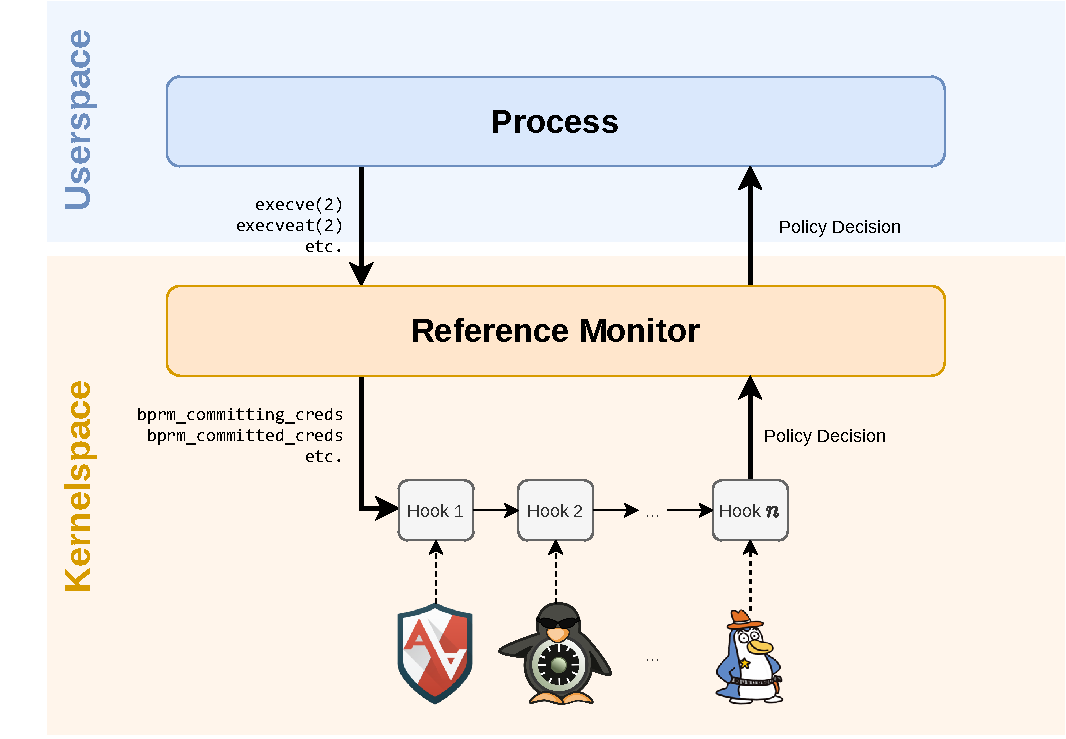
\includegraphics[width=0.8\linewidth]{figs/lsm.pdf}
    \caption{The LSM architecture. Note the many-to-many relation between access
    requests and hook invocations. Multiple LSM hooks may be chained together,
    incorporating policy from many security mechanisms. All hooks must agree to
    allow the access or it will be denied.}%
    \label{fig:lsm}
\end{figure}

The LSM API sits at a level of abstraction just above the system call API---a single LSM hook may cover multiple system calls and a single system call may contain multiple such LSM hooks. For instance, the \texttt{execve(2)} and \texttt{execveat(2)} calls both result in a call to the \texttt{bprm\_committing\_creds} and  \texttt{bprm\_committed\_creds} hooks (among others).  This provides a nice level of abstraction compared to system-call-based approaches like seccomp-bpf \cite{seccomp_bpf, drewry2012_seccomp_bpf} in that a single LSM hook can cover all closely related security events (recall the issue of \texttt{open(2)} vs.~\texttt{openat(2)} in seccomp-bpf).

The Linux kernel contains several in-tree LSM-based security modules, which may be enabled by default on certain distributions.  Many such modules implement \textit{mandatory access control} (MAC) schemes, which enable fine-grained access control that can limit the privileges of \textit{all users}---even the superuser. SELinux \cite{smalley2001_selinux} and AppArmor \cite{cowan2000_apparmor} are two such MAC LSMs, each with its own policy semantics. I discuss each in turn.

SELinux \cite{smalley2001_selinux} was originally developed by the NSA as a Linux implementation of the Flask \cite{spencer1999_flask} security model.  Under SELinux, system subjects (users, processes, etc.) and system objects (files, network sockets, etc.) are assigned corresponding labels. Security policy is then written based on these labels, specifying the allowed access patterns between a particular object type and subject type. SELinux's policy language is famously arcane \cite{schreuders12_towards}. Despite multiple efforts to introduce automated policy generation \cite{audit2allow, macmillan07_madison, sniffen06_guided}, writing and auditing SELinux security policy remains a task for security experts rather than end-users. Further, due to the difficulty of writing and auditing the complex SELinux policy language, there is a natural tendency for human policy authors to err on the side of over-permission, violating the principle of least privilege.

AppArmor (originally called SubDomain) \cite{cowan2000_apparmor} is often touted as a more usable alternative to SELinux, although usability studies have shown that this claim merits scrutiny \cite{schreuders12_towards}. Rather than basing security policy on labelling system subjects and objects, AppArmor instead employs path-based enforcement. AppArmor defines policy in per-application profiles, which contain rules specifying what system objects the application can access. System objects are identified directly (for example, via pathnames, socket classes, or IP network addresses) rather than labelled.  AppArmor also supports the notion of \textit{changing hats}, wherein a process may change its AppArmor profile under certain conditions specified in the policy.  Although AppArmor profiles are more conforming to standard Unix semantics than their SELinux counterparts, users who wish to write AppArmor policy still require a considerable amount of knowledge about operating system security \cite{schreuders12_towards}.

\subsection{Containers}
\label{subsection:containers}

Containers use OS-level virtualization and confinement mechanisms (c.f.~\Cref{subsection:low_level}) to provide a (semi-)isolated environment for the execution of processes \cite{sultan2019_container_security}. Since they run directly on the host operating system and share the underlying OS kernel, containers do not require a full guest operating system to implement virtualization. This technique has the advantage of offering a light-weight alternative to traditional hardware virtualization approaches using full virtual machines \cite{sultan2019_container_security}. Compared with containers, traditional approaches to virtualization involve hypervisors, which virtualize and provide access to the underlying hardware, either running on top of a host operating system or directly on top of the hardware itself. Full virtual machines run on top of these hypervisors, each running a guest operating system with a full userland and kernel. Full virtualization provides stronger isolation guarantees than containers but involves significantly more overhead imposed by the guest operating system \cite{sultan2019_container_security}. \Cref{fig:virt} depicts an overview of the architectural differences between containers and full hardware virtualization solutions (i.e.~virtual machines running on top of hypervisors).

\begin{figure}[htb]
  \centering
  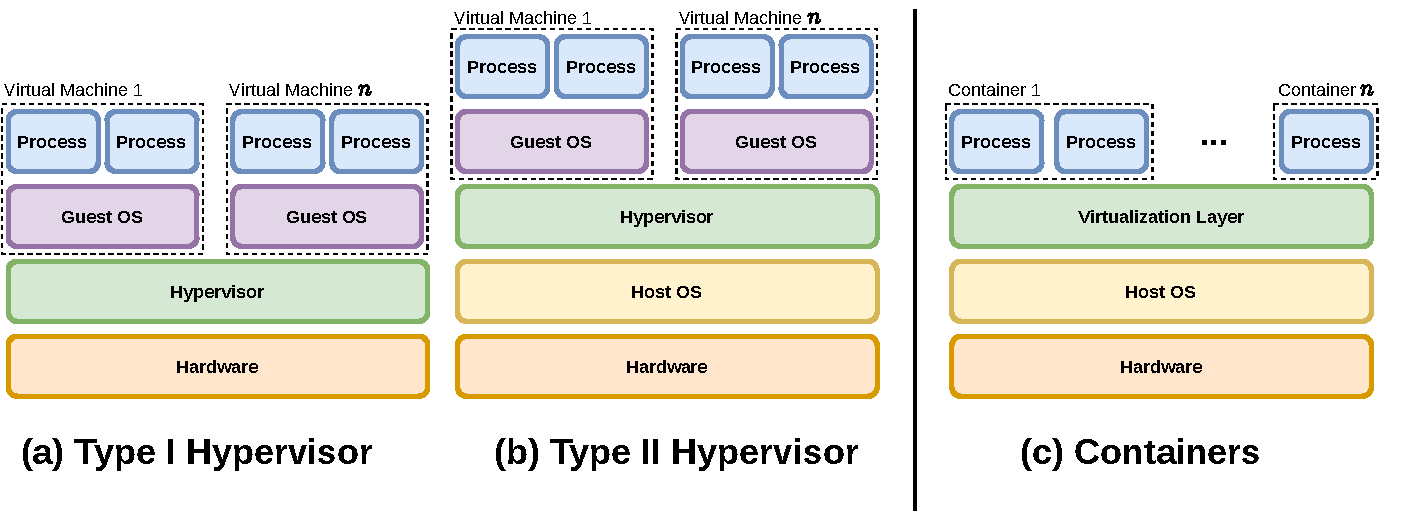
\includegraphics[width=1\linewidth]{figs/virtualization.pdf}
  \caption{
    Virtual machine and container architectures. Type I hypervisors \textbf{(a)} virtualize and control the underlying hardware directly, but require full guest operating systems on top of the virtualization layer. Type II hypervisors \textbf{(b)} run on top of a host operating system but still require full guest operating systems above the virtualization layer. Containers \textbf{(c)} achieve virtualization using a thin layer provided by the host operating system itself. They share the underlying operating system kernel and resources, and therefore require no guest operating system \cite{sultan2019_container_security}.
  }%
  \label{fig:virt}
\end{figure}

Since containers must share the host operating system kernel and related resources, it is essential to consider how best to isolate them from one another. Therefore, a container management system generally seeks to achieve the following security-related goals\footnote{Dependency management is another goal of container management systems like Docker \todo{cite}, but it is out of scope for his paper.}:
\begin{enumerate}[label=\bfseries CG\arabic*., ref=CG\arabic*, labelindent=1em]
  \item \textsc{Virtualization.}
    Virtualization aims to provide each container a \textit{virtual view} of system resources. Containers generally achieve virtualization using a combination of Linux namespaces, cgroups, and filesystem mounts. Namespaces provide a private view of enumerable resources (i.e.~a virtual mapping of IDs to resources). Such enumerable resources include process IDs, user and group IDs, mountpoints, and the network interfaces. Cgroups similarly provide a virtual view of \textit{quantifiable resources} (i.e.~how much of a given resource is available). Such quantifiable resources include the CPU, persistent storage, memory, and I/O bandwidth. Filesystem mounts, combined with mount namespaces, provide a virtual view of visible files.

    Although full virtualization may be desirable in the ideal case, containers often only implement partial virtualization \cite{sultan2019_container_security,xin2018_container_security} due to a variety of factors. Pragmatically, it is often beneficial for containers to have a shared view of specific system resources, depending on the use case. For instance, two containers might share a copy of the same shared library or require access to a shared IPC namespace to enable communication. In practice, containers often leverage layered filesystems such as overlayfs \cite{edge2010_overlayfs} to deduplicate files across containers and the host system. Partial virtualization can enable lighter-weight containers and easier communication between two containers to satisfy the goal of composability \cite{sultan2019_container_security}.

  \item \textsc{Least-Privilege.}
    For a container to be considered secure, it must enforce least-privilege on its processes \cite{sultan2019_container_security}. This requirement makes practical sense, given that a container runs directly on the host system and must share the underlying OS kernel and resources with both other containers and the host system itself. Without least-privilege, a process running in a container has virtually the same access rights as an unconfined process. When the container itself is running with privileged access to the system (as is often the case \cite{sultan2019_container_security,xin2018_container_security}), this may even result in an \textit{escalation of privilege} compared to the scenario where the process runs directly on the host. For these reasons, it is neither practical nor advisable to rely on weak virtualization guarantees to protect the host system with no means of enforcing least-privilege \cite{sultan2019_container_security}.

    A least-privilege implementation for containers typically involves a combination of multiple enforcement mechanisms, including Unix DAC, seccomp-based system call filtering, dropped POSIX capabilities, and mandatory access control mechanisms (using one of the Linux MAC LSMs) \cite{sultan2019_container_security,xin2018_container_security,docker}. This complexity can lead to usability and auditability concerns, as a simple policy language must compile down to multiple complex enforcement mechanisms that need to work cooperatively \cite{findlay2020_bpfbox}.

    Despite its evident importance for container security, existing container management solutions generally treat least-privilege as a secondary goal \cite{sultan2019_container_security}. Docker attempts to provide sensible security defaults for containers. Still, these defaults may be easily overridden and often rely on the presence of extra kernel security features such as the AppArmor LSM \cite{docker}. When AppArmor is not available, Docker falls back to relying exclusively on its default seccomp policy and dropped capabilities. Security defaults for containers also often do not adhere to the principle of least privilege. For instance, Docker provides containers with 15 Linux capabilities by default, including \texttt{CAP\_DAC\_OVERRIDE}, which allows a container to override all discretionary access control checks \cite{sultan2019_container_security,docker}.

  \item \label{item:composability} \textsc{Composability.}
    Increasingly, containers are being used to implement composable microservices \cite{sultan2019_container_security}. For instance, Kubernetes \cite{kubernetes} allows the user to group containers into \textit{pods}, which are then allowed to communicate with each other in pre-defined ways. For composability, a container needs to be able to communicate with another container without sacrificing virtualization or least-privilege. In practice, containers achieve such composability by defining specific inter-container exceptions to virtualization and least-privilege policy \cite{sultan2019_container_security}. Naturally, these exceptions can increase the risk of an insecure configuration and the user must carefully manage them to avoid overprivilege.
\end{enumerate}

\todo{Discuss prominent examples: Docker, Kubernetes}

\todo{Discuss containerized package management: Snap, FlatPak}

\subsection{Classic and Extended BPF}

The original Berkeley Packet Filter (BPF) \cite{mccanne1993_bpf}, hereafter referred to as Classic BPF, was a packet filtering mechanism implemented initially for BSD Unix. Classic BPF was created as a lightweight replacement for traditional packet filtering mechanisms, which relied on frequent context switches between userspace and kernelspace while making filtering decisions. Instead, Classic BPF implemented a simple register-based virtual machine language and efficient buffer data structures to minimize the required context switches. As an efficient packet filtering mechanism, Classic BPF quickly gained traction in the *NIX community and was subsequently ported to various open-source Unix and Unix-like operating systems, most notably Linux \cite{linux_bpf}, OpenBSD \cite{openbsd_bpf}, and FreeBSD \cite{freebsd_bpf}.

The Linux kernel development community eventually realized that the BPF engine could be applied to more than just packet filtering. The 2012 introduction of seccomp-bpf \cite{drewry2012_seccomp_bpf,seccomp_bpf} enabled Classic BPF programs to be written and applied to make system call filtering decisions for userspace applications. This extension to seccomp transformed it into a powerful (yet notoriously difficult-to-use \cite{anderson2017_comparison}) mechanism for making security decisions about system calls in a confined process.

In 2014, Starovoitov and Borkmann merged a complete rewrite of the Linux BPF engine, dubbed Extended BPF (eBPF), into the mainline kernel \cite{starovoitov2014_ebpf}. eBPF expands on the original BPF specification by introducing:
\begin{itemize}
  \item An extended instruction set;
  \item 11 registers (10 of which are general-purpose);
  \item Access to allow-listed kernel helpers;
  \item Just-in-time (JIT) compilation to native instruction sets;
  \item A program safety verifier;
  \item A large collection of specialized data structures; and
  \item New program types which can be attached to a variety of system events in both userspace and kernelspace.
\end{itemize}
These extensions to the Classic BPF engine effectively turn eBPF into a general-purpose execution engine in the kernel with powerful system introspection and kernel extension capabilities. eBPF programs execute in the kernel with supervisor privileges but are limited by a restricted execution context and pre-checked for safety by an in-kernel verification engine. In particular, eBPF programs are limited to a 512-byte stack, cannot access unbounded memory regions, must not have back-edges in their control flow, and must provably terminate \cite{gregg2019_bpf}. As a consequence of these restrictions, eBPF programs are not Turing-complete. Where necessary, an eBPF program can make calls to a set of allow-listed kernel helpers to obtain additional functionality, such as access to external memory regions and various kernel facilities such as signalling or random number generation \cite{gregg2019_bpf}.

\begin{figure}[htb]
  \centering
  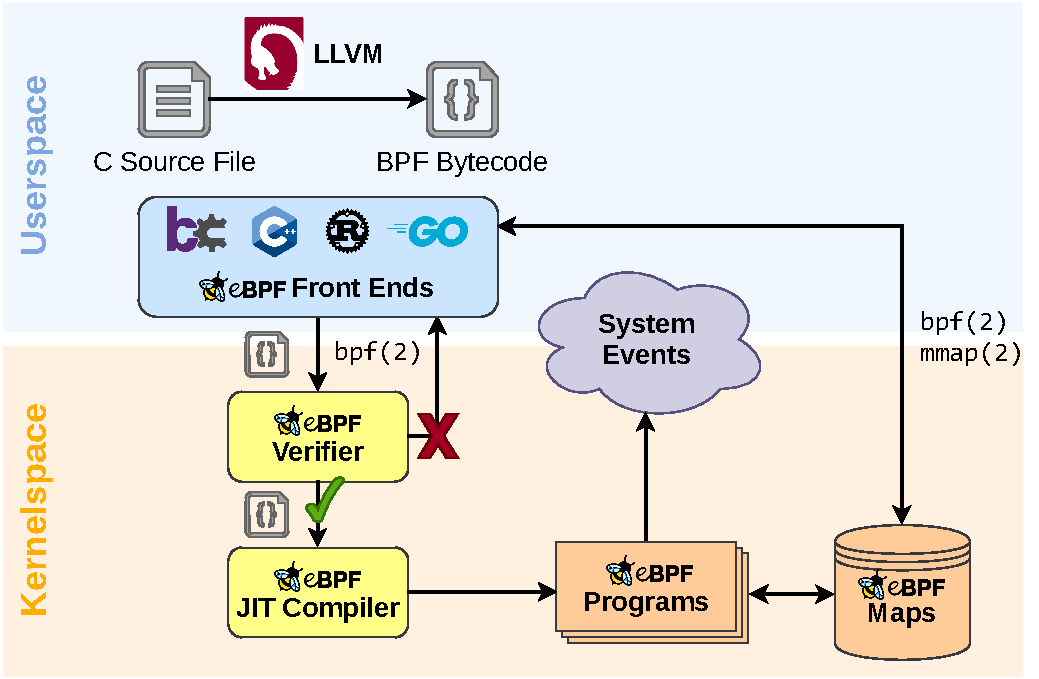
\includegraphics[width=0.8\linewidth]{figs/ebpf.pdf}
  \caption{
    eBPF mechanisms in the kernel. Userspace front-ends compile C source code into eBPF bytecode using the LLVM toolchain and load it into the kernel with the \texttt{bpf(2)} system call. The in-kernel verifier either accepts or rejects the program based on its adherence to safety invariants. Accepted programs are attached to system events across the userspace and kernelspace boundary where they are just-in-time compiled to the native instruction set. Programs can store and fetch data using data structures called \enquote{eBPF maps} which can also be accessed directly from userspace.
  }%
  \label{fig:ebpf}
\end{figure}

A privileged userspace process may load an eBPF program into the kernel using Linux's \texttt{bpf(2)} system call. While it is possible to write eBPF bytecode by hand \cite{gregg2019_bpf}, several front-ends exist for compiling eBPF bytecode from a restricted subset of the C programming language\footnote{In principle, this language need not be C. For instance, a framework exists for writing eBPF programs in pure Rust \cite{redbpf}. However, C is a popular choice since it is tightly coupled with the underlying implementation of the kernel.}, including bcc \cite{bcc} and libbpf \cite{libbpf}. These front-ends typically use the LLVM \cite{llvm_bpf} compiler toolchain to produce BPF bytecode. When the kernel receives a request to load an eBPF program, it first checks the bytecode to ensure that it conforms to the safety invariants outlined above. If the verifier accepts the program, it may then be attached to one or more system events. When an event fires, the eBPF program is executed via just-in-time compilation to the native instruction set. eBPF programs can store data in several specialized in-kernel data structures, which are also made accessible to userspace via the \texttt{bpf(2)} system call or a direct memory mapping. \Cref{fig:ebpf} depicts this process in detail.

